\begin{figure}[htpb!]
\centering
\begin{subfigure}{.5\textwidth}
  \centering
  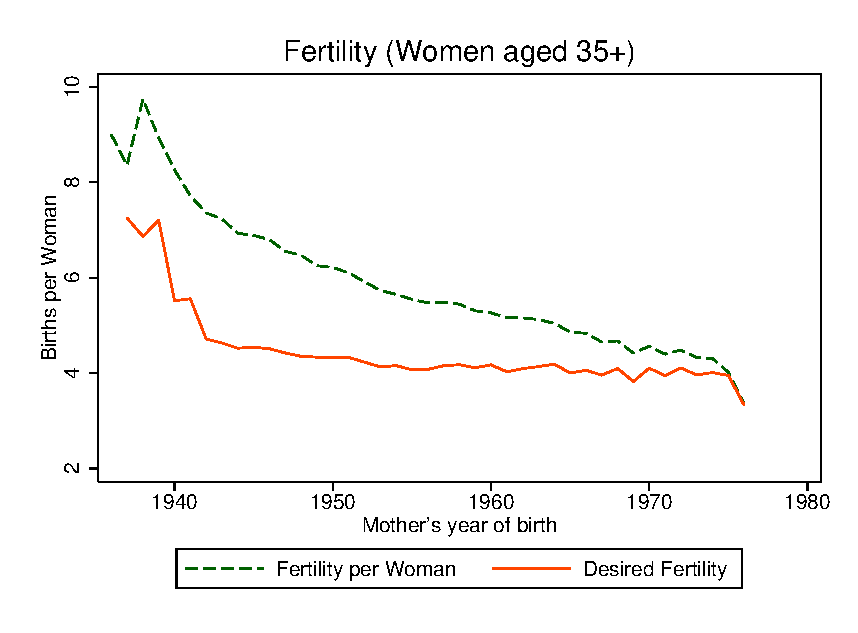
\includegraphics[scale=0.53]{\twinfolder/Figures/ferttrend_35_all.eps}
  \caption{Trends in Fertility}
  \label{TWINfig:fertrend}
\end{subfigure}%
\begin{subfigure}{.5\textwidth}
  \centering
  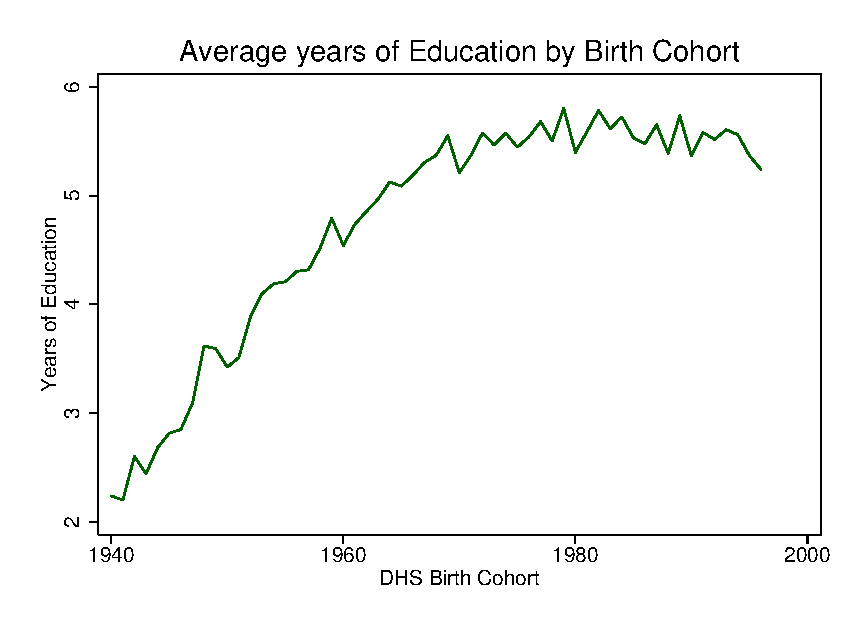
\includegraphics[scale=0.52]{\twinfolder/Figures/eductrend_all.eps}
  \caption{Trend in Education}
  \label{TWINfig:eductrend}
\end{subfigure}
\caption{Education and Fertility}
\label{TWINfig:trends}
\floatfoot{Note to figure \ref{TWINfig:trends}: Cohorts are made up of all individuals 
from the DHS who are over 35 years (for fertility), and over 15 years (for education).  
In each case the sample is restricted to those who have approximately completed fertility 
and education respectively.}
\end{figure}
\vspace{1cm}

\begin{figure}[htpb!]
\begin{center}
\caption{Twin Births and Total Fertility}
\label{TWINfig:births}
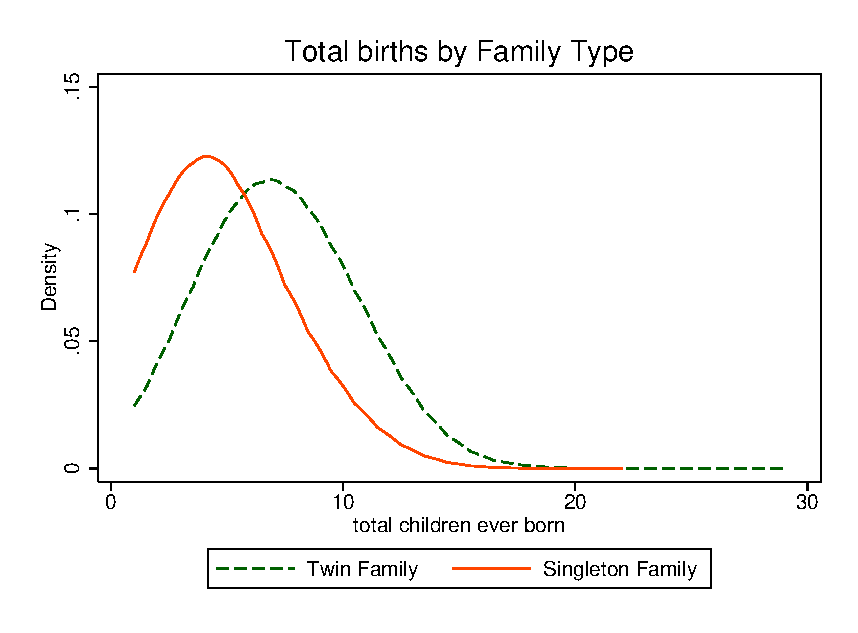
\includegraphics[scale=0.92]{\twinfolder/Figures/famsize.eps} 
\end{center}
\end{figure}

\begin{figure}[htpb!]
\begin{center}
\caption{Intra- and Inter-country trends: height and twinning}
\label{TWINfig:arrows}
\includegraphics[scale=0.86]{\twinfolder/Figures/height_country.eps} 
\end{center}
\end{figure}

\begin{figure}[htpb!]
\begin{center}
\caption{Proportion of Twins of All Births (USA)}
\label{TWINfig:USTwin}
\includegraphics[scale=0.92]{\twinfolder/Figures/USTwinFLE.eps} 
\end{center}
\end{figure}


\begin{figure}[htpb!]
\begin{center}
\caption{Plausibly Exogenous Bounds: School Z-Score (Developing Countries)}
\label{TWINfig:PEx-DHS}
\begin{subfigure}{.5\textwidth}
  \centering
  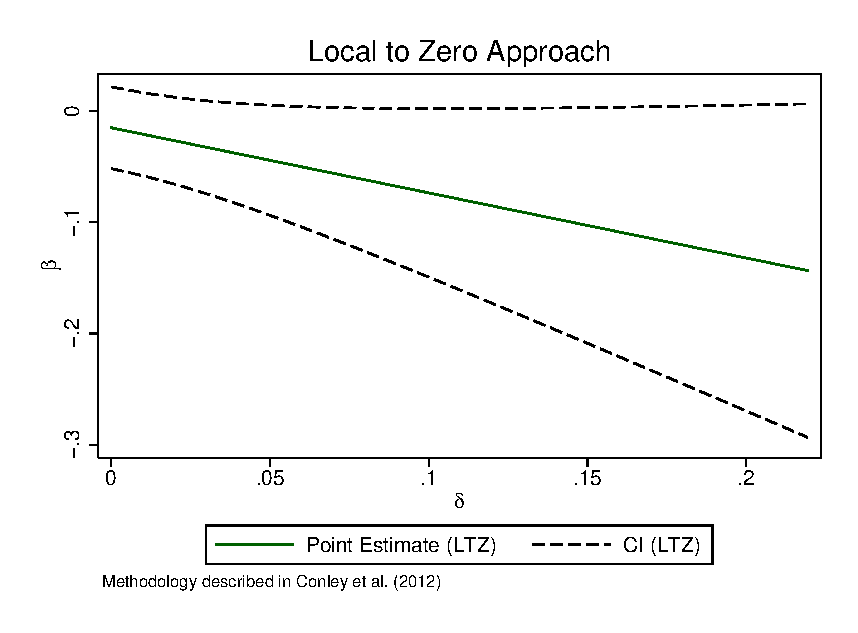
\includegraphics[scale=0.5]{\twinfolder/Figures/LTZ_two.eps}
  \caption{Two Plus}
  \label{TWINfig:ltz2}
\end{subfigure}%
\begin{subfigure}{.5\textwidth}
  \centering
  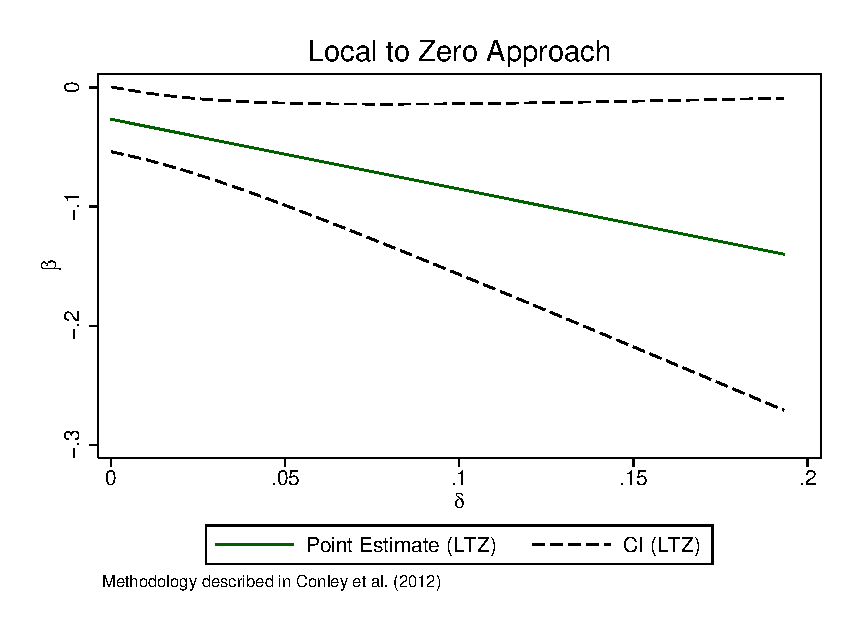
\includegraphics[scale=0.5]{\twinfolder/Figures/LTZ_three.eps}
  \caption{Three Plus}
  \label{TWINfig:ltz3}
\end{subfigure}
\end{center}
\floatfoot{Note to figure \ref{TWINfig:PEx-DHS}: Confidence intervals and point estimates 
are calculated according to \citet{Conleyetal2012}.  Estimates reflect a range of priors 
regarding the validity of the exclusion restriction required to consistently estimate 
$\hat\beta_{fert}$ using twinning in a 2SLS framework.  The local to zero (LTZ) 
approach applied here assumes that $\gamma$, the sign on the instrument when included
in the first stage, is distributed $\gamma\sim U(0,\delta)$.  The vertical dashed line
indicates 2$\times\hat\gamma$, the point at which the estimate for $\gamma$ lies 
precisely halfway between [0,$\delta$]. Further discussion is provided in appendix
\ref{TWINscn:gamma} and table \ref{TWINtab:Conley}.}
\end{figure}



\begin{figure}[htpb!]
\begin{center}
\caption{Plausibly Exogenous Bounds: School Z-Score (USA)}
\label{TWINfig:PEx-USA}
\begin{subfigure}{.5\textwidth}
  \centering
  \includegraphics[scale=0.5]{\twinfolder/Figures/ConleyUSA_EducationZscore_two.eps}
  \caption{Two Plus}
  \label{TWINfig:PEx-USA2}
\end{subfigure}%
\begin{subfigure}{.5\textwidth}
  \centering
  \includegraphics[scale=0.5]{\twinfolder/Figures/ConleyUSA_EducationZscore_three.eps}
  \caption{Three Plus}
  \label{TWINfig:PEx-USA2}
\end{subfigure}
\end{center}
\floatfoot{\textsc{Notes to figure \ref{TWINfig:PEx-USA}}: See notes to figure
\ref{TWINfig:ltz3}.}
\end{figure}

\begin{figure}[htpb!]
\begin{center}
\caption{Plausibly Exogenous Bounds: Excellent Health (USA)}
\label{TWINfig:HPEx-USA}
\begin{subfigure}{.5\textwidth}
  \centering
  \includegraphics[scale=0.5]{\twinfolder/Figures/ConleyUSA_excellentHealth_two.eps}
  \caption{Two Plus}
  \label{TWINfig:HPEx-USA2}
\end{subfigure}%
\begin{subfigure}{.5\textwidth}
  \centering
  \includegraphics[scale=0.5]{\twinfolder/Figures/ConleyUSA_excellentHealth_three.eps}
  \caption{Three Plus}
  \label{TWINfig:HPEx-USA2}
\end{subfigure}
\end{center}
\floatfoot{\textsc{Notes to figure \ref{TWINfig:HPEx-USA}}: See notes to
figure \ref{TWINfig:ltz3}.}
\end{figure}

